\section{Introduction}
	\paragraph{}{
	This chapter will outline the implementation and testing process adopted during the project. This will include information on how each component was implemented as well as any issues that occurred during the project and how they were resolved.
	}
\section{Development Environment}{
	\paragraph{}{
	Before starting implementation, a suitable development environment was required. This included a Windows 10 development PC and a method of simulating connection to a vehicle. 
	}
	\paragraph{}{
	A development PC running Windows 10 was required as part of the development environment. It was also preferable that the PC had a touchscreen, to allow testing of gesture controls, such as swipe and pinch, without deploying to a tablet. Fortunately, a Windows 8.1 touchscreen laptop which was eligible for a free Windows 10 upgrade was available before the project began. After the development PC was set up, a suitable Windows 10 tablet to deploy the application on was found. This was a low to middle end tablet, representing what an average user may own.
	}
	\paragraph{}{
	In order to be able to test the application, it needed to connect to and communicate with a vehicle. However, this was not practical as it would require moving from the development environment to the vehicle when testing or debugging the application. Initially, an application that simulated connection to an ECU was bought and used. However, during development it became evident that this would not be suitable for the project. Details about the application and why it was not suitable is discussed in section \ref{ssec:SimSoftware}.
	}
	
	\paragraph{}{
	Instead, an ECU test bench was created (see figure \ref{fig:TestBench}) that could be used as part of the development environment. This consisted of an ECU from a Rover 75 with an OBDII port and a power supply. A specific wiring diagram for the ECU had to be acquired in order to connect the wires to the corresponding pins on the ECU and OBDII port. The ECU test bench can be expanded with additional ECUs to facilitate the testing of communications with multiple communication protocols and vehicle manufacturers.
	}	
	
	\begin{figure}[h]
		\begin{center}										
				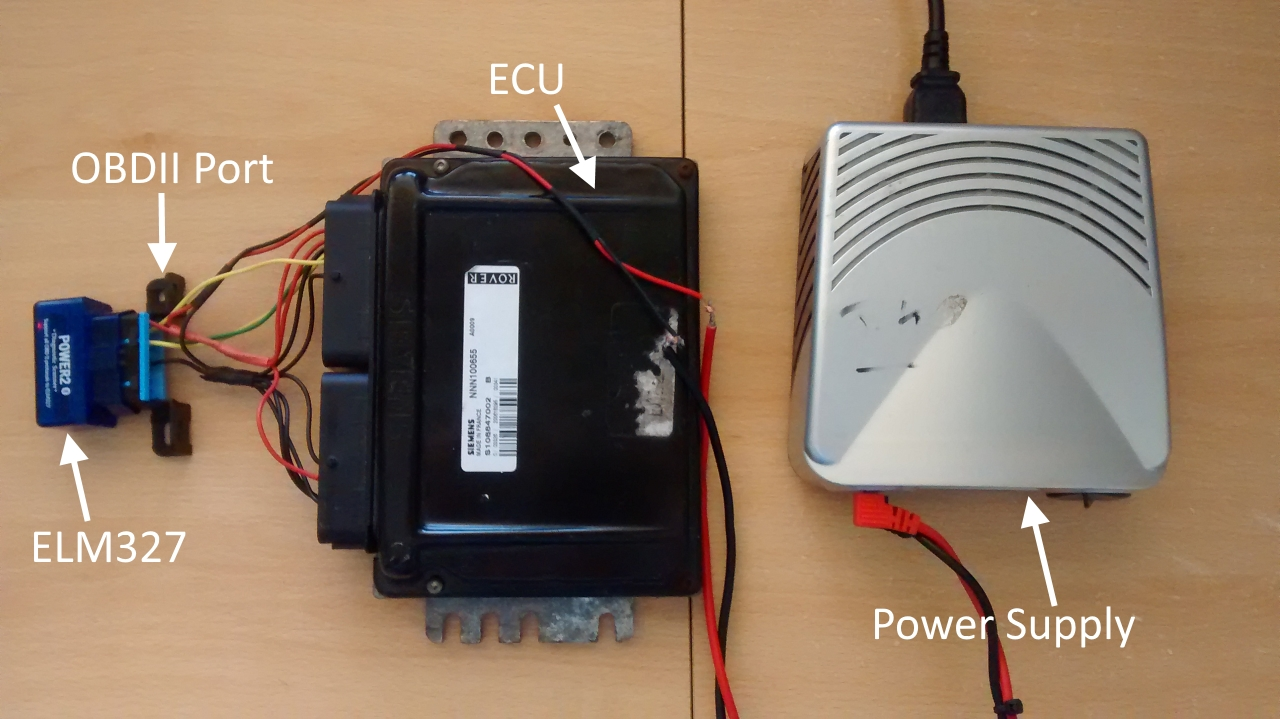
\includegraphics[width=0.8\textwidth]{ECUDesk.jpg}
				\caption{ECU test bench}
				\label{fig:TestBench}
		\end{center}
	\end{figure}
}
\label{sec:DeveEnv}

\section{Prototyping}
	\paragraph{}{
	Prior to starting the project, a lightweight proof of concept was created. This was a C{\#} console application that could connect to an ELM327 simulation application, and display live data on the screen. 
	}
	\paragraph{}{ %Bluetooth API, CAN only
	The application used the 32Feet API by In The Hand Ltd. to handle Bluetooth communication with the ELM327 simulator. The communication system was low level, as it required the address of the laptop and simulator to establish a connection. This was more low level than anticipated and resulted in the hard-coding of the addresses of the development laptop and simulator into the application, which was not optimal. One of the advantages of the 32Feet API, is that the developer can pair Bluetooth devices within their own application. However, this may also be a security issue as an incompatible or harmful device may be paired without the end user's knowledge.
	}
	\paragraph{}{
	The ELM327 simulation software used was an Android application called ECU Engine Pro. The application simulates an ELM327 device connected to an ECU using the CAN protocol. The user can manually add up to six DTCs, and can access the VIN and a limited number of PIDs, such as engine speed. The application displays the address to establish connection via Bluetooth, then the user is taken to the control panel, where they can monitor incoming and outgoing communication logs, as well as edit the DTCs and PID values being returned.
	}
	\paragraph{}{
	The application established communications with the simulator and configured the ELM327 device to use the CAN protocol using the pre-defined commands. The application would then display the first DTC as well as the current engine speed. The values that were displayed were the result of the formatting and converting of the raw data from the simulator.
	}
	\paragraph{}{	
	Overall, the prototype was a success, as it was able to display a DTC as well as the current engine speed on screen. This provided an insight into how communication and data conversion was handled, as well as how to configure the ELM327 device.
	}

\section{Bluetooth Communication}
	\subsection{Description}
		\paragraph{}{
		As the prototype had implemented a subset of the functionality for the communication, it was initially thought that this code code be updated and expanded to create the Bluetooth connection layer. However, during the development process, two key issues became evident, as detailed in section \ref{ssec:BluetoothAPI}. Firstly, the 32Feet Bluetooth API was not supported for UWP applications. Secondly, while UWP applications have their own Bluetooth API, it does not work with the ELM327 simulation software.
		%Implementation of the Bluetooth communication layer of the application began immediately after the setup of the development environment. The goal of this stage was to implement generic Bluetooth communication, such as establishing a connection with the ELM327 device and configuring it, rather than working on module specific communication, such as converting responses. The configuration steps involved resetting the device, allowing the device to auto-detect the communication protocol, turning off echoing of messages and allowing for long responses.
		}
		\paragraph{}{
		Due to these issues, the Bluetooth connection code had to be fully rewritten. This provided some benefits, as the new API is not as low level as the previous one. As seen in figure \ref{code:BTConnectionInit}, connection only requires a device ID, rather than an address of the device and the PC. Another key difference with this API is that the developer can not pair devices through the application. Instead, the user has to pair the device manually before using the application. While this was initially viewed as a limitation, it improved the security of the application, as harmful or incompatible devices cannot be paired with the user's PC. 
		%not as low level as the previous API, More secure
		}
		
		\begin{figure}[h]
			\begin{lstlisting}
// Set up a service for the Bluetooth device
this.service = await RfcommDeviceService.FromIdAsync(this.CurrentDevice.Id);

if (this.service != null)
{
	this.DeviceConnectionStatus = ConnectionStatus.Connecting;
	this.socket = new StreamSocket();

	// Timeout after 5 seconds
	CancellationTokenSource token = new CancellationTokenSource();
	token.CancelAfter(5000);

	try
	{
		// Connect to the socket
		await socket.ConnectAsync(this.service.ConnectionHostName,this.service.ConnectionServiceName, SocketProtectionLevel.BluetoothEncryptionAllowNullAuthentication).AsTask(token.Token);
	
		// Set up the reader and writer using the socket input stream and output stream respectively
		this.writer = new DataWriter(this.socket.OutputStream);
		this.reader = new DataReader(this.socket.InputStream);    		
	}
	catch(TaskCanceledException e)
	{
		this.DeviceConnectionStatus = ConnectionStatus.NotConnected;                            
	}
}
			\end{lstlisting}
			\caption{Establishing a connection to the ELM327}
			\label{code:BTConnectionInit}
		\end{figure}

		\paragraph{}{
		The main component of the Bluetooth connection system was sending and receiving data. As seen in figure \ref{code:BTConnectionSend}, a command is sent to the data writer and appended with a return carriage, to inform the ELM327 that the command has terminated. The reader then attempts to read any incoming messages. However, the length of the  message is unknown and can vary for each command. To deal with this the reader reads one character at a time until a '\textgreater' character appears, signifying the end of the message. If the reader cannot read the entire message, for example, if the user walks out of range of the device, or removes it from the vehicle, the connection will time out.
		% Send & Receive, don't know length of response
		}

		\begin{figure}[h]
			\begin{lstlisting}
// Write
if (this.writer != null)
{
    this.writer.WriteString(command + "\r");
	await this.writer.StoreAsync();
}

// Timeout after 5 seconds                
CancellationTokenSource token = new CancellationTokenSource();
token.CancelAfter(5000);

// Read
try
{
	while (!response.Contains(">"))
	{
		uint size = await this.reader.LoadAsync(1).AsTask(token.Token);                        
        string s = this.reader.ReadString(size);
		response += s;
	}
    
    response = response.Replace(">", "");
}
catch (Exception e)
{
	// Shutdown communication on timeout
	response = NO_CONNECTION;
	this.IsInitialized = false;
}                

if (response.Contains("UNABLE TO CONNECT"))
{
	// Shutdown communication on unable to connect
	response = NO_CONNECTION;
    this.IsInitialized = false;
}

return response;
			\end{lstlisting}
			\caption{Sending a command to the ELM327 and receiving a response}
			\label{code:BTConnectionSend}
		\end{figure}		
		
		%\paragraph{}{
		%There were some issues with the 32Feet Bluetooth API, outlined in section 5.5.1, that lead to the use of Microsoft's own Bluetooth API in it's place. This API allows developers to find all Bluetooth device paired with the PC and choose the appropriate one from the list. Due to the use of this new API, there was less time to work on Bluetooth communication, so the application was created to connect to the first suitable Bluetooth device on the network, with the intention of adding a search function at a later date.
		%}
	\subsection{Issues}
		\subsubsection{Issue 1: Bluetooth API}{
			\paragraph{Description:}
			The 32Feet Bluetooth API used in the prototype was incompatible with the UWP application. This meant that the prototype code that was written for Bluetooth connection could not be reused in the final product.
				
			\paragraph{Occurred during:}
			Week 1
		
			\paragraph{Time taken to resolve:} Half a week to identify the issue, one week to find an alternative solution and one week to implement this solution.
		
			\paragraph{Attempts to resolve:}
			A number of attempts to resolve the issue were made, such as searching for newer versions of the API and researching potential workarounds. Unfortunately, it became evident that the API was completely incompatible with UWP applications, leading to a stand still in development until a replacement could be found.
			
			\paragraph{Solution:}
			Microsoft includes their own Bluetooth API with UWP and this was chosen as a replacement for the 32Feet Bluetooth API. There was an unexpected learning curve that affected the project timeline, but this solution ultimately improved the security of the application and decreased the complexity of the code.
		}
		\label{ssec:BluetoothAPI}
		
		\subsubsection{Issue 2: Simulation software}{
			\paragraph{Description:}
			The replacement Bluetooth API could not connect to the ECU simulation software. This meant connection to an actual vehicle was required to debug and test the application.
			
			\paragraph{Occurred during:}
			Week 1
			\paragraph{Time taken to resolve:}
			One week to find a workaround and half a week to set up ECU.
			\paragraph{Attempts to resolve:}
			Several attempts to contact the developer were made through emails and the Google Play Store, where the application was bought. Unfortunately, no response was received and a decision was reached that the application could not be utilised for this project, as it seemed highly unlikely that the application would be updated to support the Bluetooth API. 
%Looked for other apps
			\paragraph{Solution:}
			To simulate connection to a vehicle, an ECU test bench was created as outlined in section \ref{sec:DeveEnv}. This had an impact on the timeline of the project, as a number of components, such as an ECU and a wiring diagram, had to be sourced as well as assembling the test bench itself. Ultimately, the ECU test bench had the advantage of extensibility over the ECU simulation software, as the latter only supported one protocol, whereas the former can be extended with new ECUs that support various protocols.
		}
		\label{ssec:SimSoftware}		

\section{DTC Module}
		\paragraph{}{
		%Implementation of the DTC module involved creating a UI layer, a module layer and a communication layer for DTCs.	Initially, the DTC module was implemented to only retrieve and display one DTC of each type. This was to quickly test the functionality of the communication system and to provide an impression of the general aesthetics of the module, before implementing it in its entirety.
		}		
		\paragraph{}{
		%The core functionality of this module was to request all current, pending and permanent DTCs and display them on screen grouped by their types. Initially, the module requested current DTCs, and only converted and displayed the first DTC from the response. This code was then reworked to display the first pending DTC and the first permanent DTC. Once the user interface was fully implemented, the module was rewritten to display all DTCs.
		}
		\paragraph{}{
		%Another key aspect of this module was the implementation of the clear codes functionality. The module included a button that, when pressed, issued the clear codes command, then acquired the new list of DTCs and refreshed the UI.
		}
		\paragraph{}{
		%[DTC Info issue]
		}
		
\section{Simulated Communication}
		\paragraph{}{
		While preparing to implement the data module, a potential problem was discovered. While the ECU test bench sent back data that could be graphed, the values were static and could not be changed. This would make it difficult to test the data graphing, as it would require communication with a live vehicle to gather dynamic data values. Instead, a simulation connection class was created.
		%[Preparation for data module, acts like an ECU, behaves like real world (time, responses etc)]
		}
		\paragraph{}{
		The simulation connection class implements the IDataConnection interface seen in figure \ref{code:ConnectionInterface}, but instead of connecting to a Bluetooth device, it handles the requests and returns a response in the format that the ELM327 would use, sending response in hexadecimal format. Because of this, the simulation connection more accurately represents communication with a vehicle and did not require a refactor of the code in the communication layer.
		}	
		\begin{figure}[h]
			\begin{lstlisting}
string response = "NO DATA";

// Request for Data (Mode 01)
if (command.StartsWith("01"))
{
	// Get supported pids
	if (command.StartsWith("0100"))
    {
		// Binary Value: 0001 1000 0111 1000 0000 0000 0000 0000
		response = "410018580000";
	}
    else if (command.StartsWith("0104"))
	{
    	/* Conversion formula: A * 100 / 255 */
    	
    	// Generate a number between the minimum and maximum value
        int min = 0;
		int max = 100;
        Random r = new Random();
		int value = r.Next(min, max);

		// Reverse the equation and convert to hex
        value = (255 * value) / 100;
		response = "4104" + value.ToString("X2");
	}
}
			\end{lstlisting}
			\caption{Simulation connection code for 0100 and 0104 requests}
			\label{code:SimConnectionData}
		\end{figure}

		\paragraph{}{
		As shown in the code fragment seen  in figure \ref{code:SimConnectionData}, a small subset of pids are supported, and each of these pids will return data when a request is made. As each pid has a maximum and minimum possible value, a random value between these two will be generated and this will be the value that the user sees on-screen. The value  is passed through a conversion equation, in reverse order to convert it to hexadecimal format. Finally, the response header is prefixed to this hexadecimal message and is returned to the caller. A more detailed description of how these conversions work can be found in section \ref{ssec:DataModuleDesc}.
		}
		\paragraph{}{
		Due to the success of the simulation connection with respect to the data module, it was expanded to work with the DTC module, returning a set of current, pending and permanent DTCs, as seen in figure \ref{code:SimConnectionDTC}.
		}
		
		\begin{figure}[h]
			\begin{lstlisting}
// Current DTCs
if (command.StartsWith("03"))
{
	// Return P0101, P0121 and P0353	
	response = "43010101210353";
}
// Pending DTCs
else if (command.StartsWith("07"))
{
	// Return P0104, P0132 and P0342	
	response = "47010401320342";
}
// Permanent DTCs
else if (command.StartsWith("0A"))
{
	// Return P0107, P0109 and P0111	
	response = "4A010701090111";
}			
			\end{lstlisting}
			\caption{Simulation connection code for current, pending and permanent DTCs}
			\label{code:SimConnectionDTC}
		\end{figure}

\section{Data Module}
	\subsection{Description}{		
		\paragraph{}{
		[Graphs, List, Play/Pause/Step Controls, Smart Graphing]
		}
		\label{ssec:DataModuleDesc}
	}
	\subsection{Issues}{		
		\paragraph{}{
		[Speed 300ms, down to 170ms]
		[Graph blurring - Smart graphing fixed this but memory was an issue]
		}
		\label{ssec:DataModuleIssues}
	}

\section{Connection Module}
		\paragraph{}{
		[List of paired devices, connection status, comm log]
		}
	
\section{Android Port}
	\subsection{Description}		
		\paragraph{}{
		[Port preparation, MVVM, Bluetooth layer, UI]
		}	
	\subsection{Issues}{
	}
	\label{ssec:AndroidIssues}
\section{Help Information}
		\paragraph{}{
		[Moving help info out of other modules, help shouldn't interrupt modules]
		}
	
\section{Home Module}
		\paragraph{}{
		[Need to implement this]
		}
	
%\section{Performance Re-factoring}
		%\paragraph{}
		%[Module shutdown, limited pids]
		
	
%\section{Issues}
	%\paragraph{}{
	%During implementation, a number of serious issues were encountered that affected the design and development of the project. These issues were resolved, but often required a reconsideration of the initial design decisions.
	%}
	
	%\subsection{Issue 1: Bluetooth API}
		%\paragraph{Description:}
		%The 32Feet Bluetooth API used in the prototype was incompatible with the UWP application. This meant that the prototype code that was written for Bluetooth connection could not be reused in the final product.
		
		%\paragraph{Occurred during:}
		%Week 1
		
		%\paragraph{Time taken to resolve:}
		%Approximately one week
		
		%\paragraph{Attempts to resolve:}
		%A number of attempts to resolve the issue were made, such as searching for newer versions of the API and researching potential workarounds. Unfortunately, it became evident that the API was completely incompatible with UWP applications, leading to a stand still in development until a replacement could be found.
		
		%\paragraph{Solution:}
		%Microsoft includes their own Bluetooth API with UWP and this was chosen as a replacement for the 32Feet Bluetooth API. Aside from the unexpected learning curve, this solution had it's inconveniences, such as not allowing devices to be paired through the application. This meant that there was additional configuration required by the end user. However, this also created a more secure application, as the chance of automatically pairing a potentially malicious device was decreased.
		
	%\subsection{Issue 2: Simulation software}
		%\paragraph{Description:}
		%The replacement Bluetooth API could not connect to the ECU simulation software. This meant connection to an actual vehicle was required to debug and test the application.
		
		%\paragraph{Occurred during:}
		%Week 1
		
		%\paragraph{Time taken to resolve:}
		%Approximately two weeks
		
		%\paragraph{Attempts to resolve:}
		%Several attempts to contact the developer were made through emails and the Google Play Store, where the application was bought. Unfortunately, no response was received and a decision was reached that the application could not be utilised for this project, as it seemed highly unlikely that the application would be updated to support the Bluetooth API. 
		
		%\paragraph{Solution:}
		%To simulate connection to a vehicle, an ECU test bench was created as outlined in section 5.2. This had an impact on the timeline of the project, as a number of components, such as an ECU and a wiring diagram, had to be sourced as well as assembling the test bench itself. Ultimately, the ECU test bench had the advantage of extensibility over the ECU simulation software, as the latter only supported one protocol, whereas the former can be extended with new ECUs that support various protocols.
		